\begin{table}[htbp]
\centering
\caption{Comparación de Puntuaciones de Frameworks}
\label{tab:frameworks_scores}
\begin{tabular}{lc}
\toprule
\textbf{Framework} & \textbf{Puntuación} \\
\midrule
React & 9.2 \\
Vue.js & 8.9 \\
Spring Boot & 8.8 \\
Angular & 8.7 \\
Django & 8.5 \\
Express.js & 8.3 \\
Laravel & 8.1 \\
\bottomrule
\end{tabular}
\end{table}

\begin{figure}[htbp]
\centering
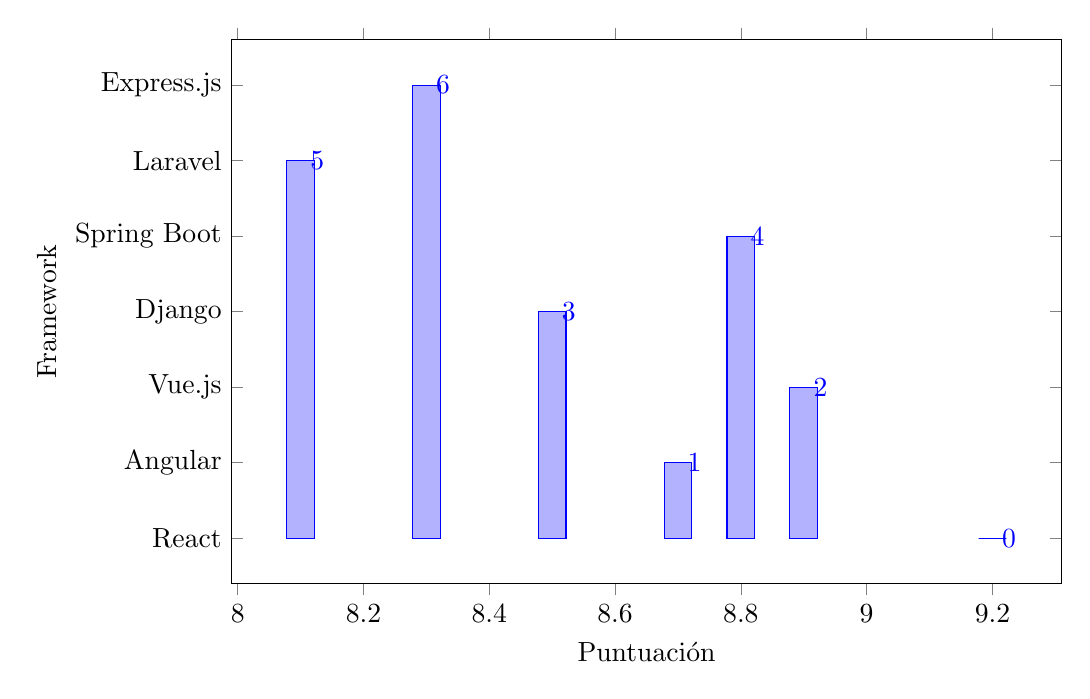
\begin{tikzpicture}
\begin{axis}[
    ybar,
    width=\columnwidth,
    height=0.7\columnwidth,
    xlabel={Puntuación},
    ylabel={Framework},
    symbolic y coords={React,Angular,Vue.js,Django,Spring Boot,Laravel,Express.js},
    ytick=data,
    nodes near coords,
    nodes near coords align={horizontal},
    enlargelimits=0.1,
]
\addplot coordinates {(9.2,React) (8.7,Angular) (8.9,Vue.js) (8.5,Django) (8.8,Spring Boot) (8.1,Laravel) (8.3,Express.js)};
\end{axis}
\end{tikzpicture}
\caption{Gráfica de Puntuaciones de Frameworks}
\label{fig:frameworks_visual}
\end{figure}